In the lecture we have derived the following 
RG flow equation for the coupling constant $K$ 
of the Ising chain without magnetic field: 
the new value $K'$ is given by
\begin{equation}
    K'(K)=\frac{1}{2}\ln\cosh(2K).
\end{equation}
In addition we have derived the absolute 
increase in free energy per spin arising in 
each iteration:
\begin{equation}
    g(K)=\frac{1}{2}\ln2
    +\frac{1}{4}\ln\cosh(2K)
\end{equation}

\paragraph{1. Write a short computer program 
    (e.g. in Mathematica or Python) that 
    defines the flow equation $K'(K)$ and the 
    free energy increase $g(K)$ as functions. 
    Start with a coupling constant $K_0=1$ and 
    iterate through $K_1$, $K_2$, $K_3$ up to 
    $K_4$. Also calculated the corresponding 
    values $g_0=g(K_0)$ to $g_4=g(K_4).$ What 
    are the limits for these two series? 
    \textit{(1.5 points)}
} \ \\
    \\
    Python functions:
    \lstinputlisting[firstline=6, lastline=11]{./code/task03a.py}
    Iteration to $i=4$ yields
    \begin{table}[h!]
        \begin{center}
        \begin{tabular}{llllll}
                  & i=0  & i=1  & i=2  & i=3  & i=4  \\ 
            \hline
            $K_i$ & 1    & 0.66 & 0.35 & 0.11 & 0.01 \\ 
            $g_i$ & 0.68 & 0.52 & 0.4  & 0.35 & 0.35 \\ 
        \end{tabular}
        \end{center}
    \end{table} \ \\ 
    The $K_i$-series converges to zero for 
    large $i$, while the $g_i$-series 
    converges to $\frac{1}{2}\ln2\approx0.35$.
    \begin{figure}[h!]
        \centering
        \begin{minipage}{.5\linewidth}
          \centering
          \subfloat[coupling constant $K$]{
            \label{:a}
            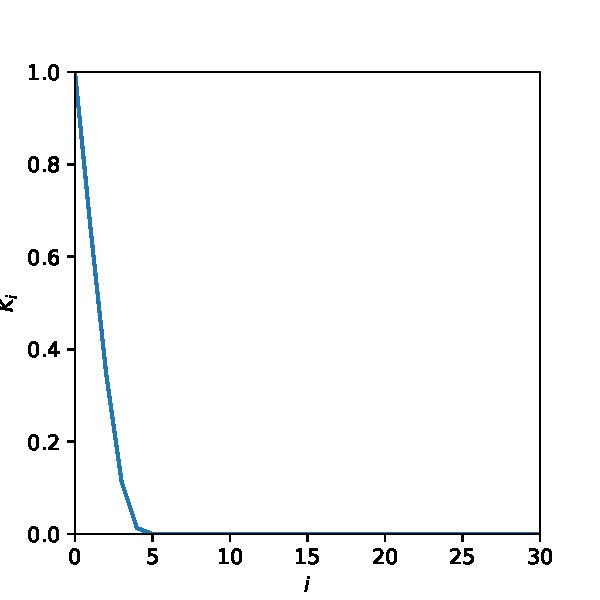
\includegraphics[scale=.7]{./figures/K_series.pdf}
          }
        \end{minipage}%
        \begin{minipage}{.5\linewidth}
          \centering
          \subfloat[free energy increase $g$]{
            \label{:b}
            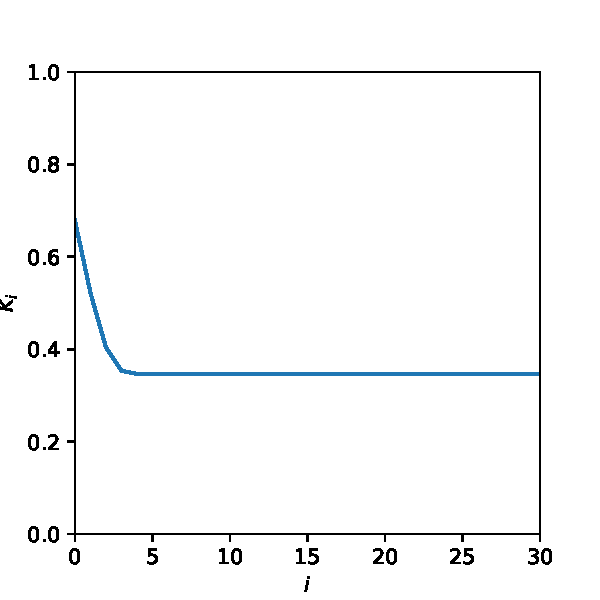
\includegraphics[scale=.7]{./figures/g_series.pdf}
          }
        \end{minipage}
    \end{figure} \ \\


\paragraph{2. Use these results to estimate 
    the dimensionless free energy per spin 
    $f=-\beta F/N$ in fourth order (simply cut 
    the appropriate sum after the term with 
    $g_4$; you can also include the next order
    term, but now by simply using the first 
    term in $g(K)$). Compare to the known 
    exact result for the Ising chain. How good
    is the numerical agreement?
    \textit{(1.5 points)}
}
    \begin{align}
        f
        &=\sum_{i=0}^{4}g_i
        \approx2.3
    \end{align}
